\section{Modelo Entidad-Relación}
El modelo entidad-relación describe la estructura lógica del sistema \textbf{QuickContentMedia},  identificando las principales entidades, sus atributos y las relaciones existentes entre ellas. 

\subsection{Diagrama del modelo entidad-
relación}
La figura \ref{fig:MER} presenta el diagrama del modelo entidad-relación. Este modelo sirve como base para el posterior diseño de la base de datos relacional. Este modelo fue elaborado utilizando la herramienta TerraER.

\begin{figure}[H]
    \centering
    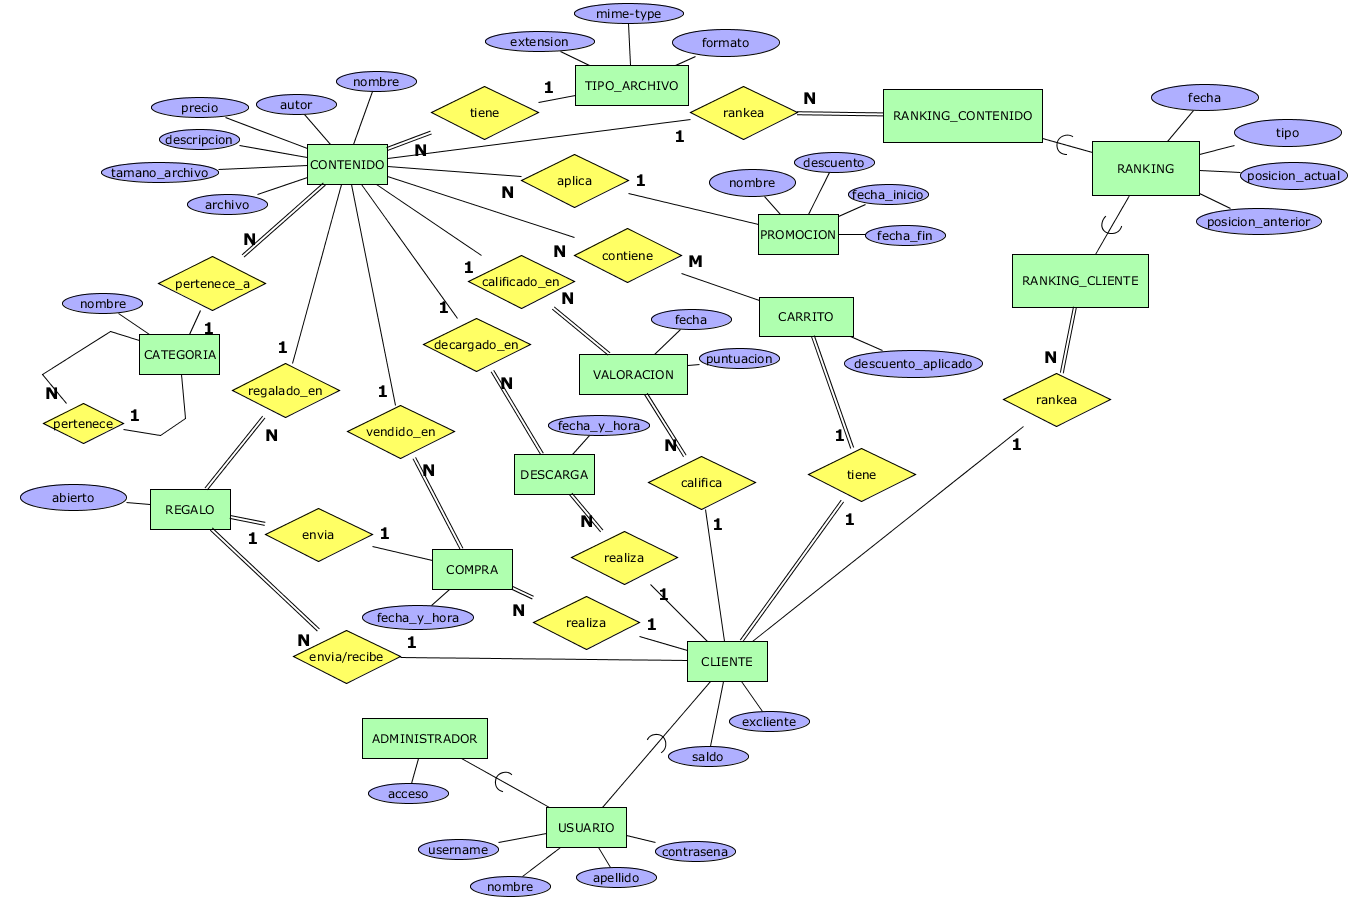
\includegraphics[width=1\linewidth]{Media/3_Analisis/3_ModeloEntidadRelacion/MER.png}
    \caption{Modelo entidad-relación (MER-001) del sistema QuickContentMedia}
    \label{fig:MER}
\end{figure}

\textbf{Archivo:} {Modelo entidad-relación} \\
\textbf{Link de acceso:} \linkMER \\

\textbf{Pasos de ejecución:}
\begin{itemize}
    \item Ingresar al repositorio en GitHub usando el link proporcionado y descargar el archivo MER.xml y TerraER3.14.jar
    \item Ejecutar el pograma TerraER3.14.jar
    \item En la pestaña File seleccionar la opción open y seleccionar el archivo MER.xml
\end{itemize}

\subsection{Diccionario de entidades}

El diccionario de entidades está compuesto por el nombre de la entidad, su descripción, sus atributos y sus tipos. 

% ==== Entidad USUARIO ====
\renewcommand{\arraystretch}{1.3}
\begin{longtable}{|p{3.5cm}|p{10cm}|}
\caption{Diccionario de la entidad Usuario}
\label{tab:diccionarioUsuario} \\ \hline
\textbf{Nombre:} & Usuario \\ \hline
\textbf{Descripción:} & 
Entidad que representa a cualquier persona con credenciales para iniciar sesión en el portal \textbf{QuickContentMedia}.  
Sirve como super-tipo de \textbf{Cliente} y \textbf{Administrador}. \\ \hline
\endfirsthead

\multicolumn{2}{c}{\textbf{Continuación desde la página anterior}} \\ \hline
\endhead

\hline \multicolumn{2}{r}{{Continúa en la siguiente página}} \\ \hline
\endfoot

\hline
\endlastfoot

\multicolumn{2}{|p{13.5cm}|}{\textbf{ATRIBUTOS}} \\ \hline
\textbf{Atributo} & \textbf{Descripción} \\ \hline
username   & Identificador único de inicio de sesión.  
Tipo: \textit{string}. \\ \hline
contrasena & Contraseña cifrada asociada al usuario.  
Tipo: \textit{string}. \\ \hline
nombre     & Nombre de pila.  
Tipo: \textit{string}. \\ \hline
apellido   & Apellidos completos.  
Tipo: \textit{string}. \\ \hline
\end{longtable}

% ==== Entidad CLIENTE ====
\renewcommand{\arraystretch}{1.3}
\begin{longtable}{|p{3.5cm}|p{10cm}|}
\caption{Diccionario de la entidad Cliente}
\label{tab:diccionarioCliente} \\ \hline
\textbf{Nombre:} & Cliente \\ \hline
\textbf{Descripción:} & 
Sub-tipo de \textbf{Usuario} que interactúa como consumidor: compra, descarga, califica contenidos y participa en rankings. \\ \hline
\endfirsthead
\multicolumn{2}{c}{\textbf{Continuación desde la página anterior}} \\ \hline
\endhead
\hline \multicolumn{2}{r}{{Continúa en la siguiente página}} \\ \hline
\endfoot
\hline
\endlastfoot
\multicolumn{2}{|p{13.5cm}|}{\textbf{ATRIBUTOS}} \\ \hline
\textbf{Atributo} & \textbf{Descripción} \\ \hline
saldo      & Saldo disponible para compras.  
Tipo: \textit{Integer}. \\ \hline
excliente  & Indica si la cuenta se encuentra cerrada (pasa a ex-cliente).  
Tipo: \textit{boolean}. \\ \hline
\end{longtable}

% ==== Entidad ADMINISTRADOR ====
\renewcommand{\arraystretch}{1.3}
\begin{longtable}{|p{3.5cm}|p{10cm}|}
\caption{Diccionario de la entidad Administrador}
\label{tab:diccionarioAdministrador} \\ \hline
\textbf{Nombre:} & Administrador \\ \hline
\textbf{Descripción:} & 
Sub-tipo de \textbf{Usuario} con privilegios de gestión: alta/baja contenidos, creación de promociones, recarga de saldo y administración de categorías. \\ \hline
\endfirsthead
\multicolumn{2}{c}{\textbf{Continuación desde la página anterior}} \\ \hline
\endhead
\hline \multicolumn{2}{r}{{Continúa en la siguiente página}} \\ \hline
\endfoot
\hline
\endlastfoot
\multicolumn{2}{|p{13.5cm}|}{\textbf{ATRIBUTOS}} \\ \hline
\textbf{Atributo} & \textbf{Descripción} \\ \hline
acceso & Nivel o clave de acceso al módulo de administración.  
Tipo: \textit{boolean}. \\ \hline
\end{longtable}

% ==== Entidad CONTENIDO ====
\renewcommand{\arraystretch}{1.3}
\begin{longtable}{|p{3.5cm}|p{10cm}|}
\caption{Diccionario de la entidad Contenido}
\label{tab:diccionarioContenido} \\ \hline
\textbf{Nombre:} & Contenido \\ \hline
\textbf{Descripción:} & 
Archivo multimedia que el portal ofrece para descarga (imágenes, sonidos o videos) junto a sus metadatos de catalogación. \\ \hline
\endfirsthead
\multicolumn{2}{c}{\textbf{Continuación desde la página anterior}} \\ \hline
\endhead
\hline \multicolumn{2}{r}{{Continúa en la siguiente página}} \\ \hline
\endfoot
\hline
\endlastfoot
\multicolumn{2}{|p{13.5cm}|}{\textbf{ATRIBUTOS}} \\ \hline
\textbf{Atributo} & \textbf{Descripción} \\ \hline
nombre          & Título descriptivo del contenido.  
Tipo: \textit{string}. \\ \hline
autor           & Autor o creador del contenido.  
Tipo: \textit{string}. \\ \hline
descripcion     & Resumen o descripción ampliada.  
Tipo: \textit{string}. \\ \hline
precio          & Precio de venta en la moneda definida por el sistema.  
Tipo: \textit{integer}. \\ \hline
tamano\_archivo & Peso del archivo en bytes o MB.  
Tipo: \textit{double}. \\ \hline
archivo         & Datos binarios del fichero.  
Tipo: \textit{binary}. \\ \hline
\end{longtable}

% ==== Entidad TIPO_ARCHIVO ====
\renewcommand{\arraystretch}{1.3}
\begin{longtable}{|p{3.5cm}|p{10cm}|}
\caption{Diccionario de la entidad Tipo\_Archivo}
\label{tab:diccionarioTipoArchivo} \\ \hline
\textbf{Nombre:} & Tipo\_Archivo \\ \hline
\textbf{Descripción:} & 
Catálogo de extensiones y metainformación técnica de los contenidos. \\ \hline
\endfirsthead
\multicolumn{2}{c}{\textbf{Continuación desde la página anterior}} \\ \hline
\endhead
\hline \multicolumn{2}{r}{{Continúa en la siguiente página}} \\ \hline
\endfoot
\hline
\endlastfoot
\multicolumn{2}{|p{13.5cm}|}{\textbf{ATRIBUTOS}} \\ \hline
\textbf{Atributo} & \textbf{Descripción} \\ \hline
extension  & Extensión física (JPG, MP3, AVI, …).  
Tipo: \textit{string}. \\ \hline
mime\_type & Tipo MIME oficial (image/jpeg, audio/mpeg, …).  
Tipo: \textit{string}. \\ \hline
formato    & Categoría general (imagen, música, video).  
Tipo: \textit{string}. \\ \hline
\end{longtable}

% ==== Entidad CATEGORIA ====
\renewcommand{\arraystretch}{1.3}
\begin{longtable}{|p{3.5cm}|p{10cm}|}
\caption{Diccionario de la entidad Categoría}
\label{tab:diccionarioCategoria} \\ \hline
\textbf{Nombre:} & Categoría \\ \hline
\textbf{Descripción:} & 
Etiqueta dentro del árbol jerárquico que agrupa contenidos de temática similar.  Puede anidarse sin límite de profundidad. \\ \hline
\endfirsthead
\multicolumn{2}{c}{\textbf{Continuación desde la página anterior}} \\ \hline
\endhead
\hline \multicolumn{2}{r}{{Continúa en la siguiente página}} \\ \hline
\endfoot
\hline
\endlastfoot
\multicolumn{2}{|p{13.5cm}|}{\textbf{ATRIBUTOS}} \\ \hline
\textbf{Atributo} & \textbf{Descripción} \\ \hline
nombre & Nombre de la categoría.  
Tipo: \textit{string}. \\ \hline
\end{longtable}

% ==== Entidad PROMOCION ====
\renewcommand{\arraystretch}{1.3}
\begin{longtable}{|p{3.5cm}|p{10cm}|}
\caption{Diccionario de la entidad Promoción}
\label{tab:diccionarioPromocion} \\ \hline
\textbf{Nombre:} & Promoción \\ \hline
\textbf{Descripción:} & 
Descuento temporal aplicado a uno o varios contenidos. \\ \hline
\endfirsthead
\multicolumn{2}{c}{\textbf{Continuación desde la página anterior}} \\ \hline
\endhead
\hline \multicolumn{2}{r}{{Continúa en la siguiente página}} \\ \hline
\endfoot
\hline
\endlastfoot
\multicolumn{2}{|p{13.5cm}|}{\textbf{ATRIBUTOS}} \\ \hline
\textbf{Atributo} & \textbf{Descripción} \\ \hline
nombre       & Nombre identificador de la promoción.  
Tipo: \textit{string}. \\ \hline
descuento    & Porcentaje de descuento (0–100).  
Tipo: \textit{integer}. \\ \hline
fecha\_inicio & Fecha de inicio de la vigencia.  
Tipo: \textit{date}. \\ \hline
fecha\_fin   & Fecha de término de la vigencia.  
Tipo: \textit{date}. \\ \hline
\end{longtable}

% ==== Entidad REGALO ====
\renewcommand{\arraystretch}{1.3}
\begin{longtable}{|p{3.5cm}|p{10cm}|}
\caption{Diccionario de la entidad Regalo}
\label{tab:diccionarioRegalo} \\ \hline
\textbf{Nombre:} & Regalo \\ \hline
\textbf{Descripción:} & 
Representa el envío de uno o más contenidos de un cliente a otro como presente. \\ \hline
\endfirsthead
\multicolumn{2}{c}{\textbf{Continuación desde la página anterior}} \\ \hline
\endhead
\hline \multicolumn{2}{r}{{Continúa en la siguiente página}} \\ \hline
\endfoot
\hline
\endlastfoot
\multicolumn{2}{|p{13.5cm}|}{\textbf{ATRIBUTOS}} \\ \hline
\textbf{Atributo} & \textbf{Descripción} \\ \hline
abierto & Indica si el destinatario ya abrió el regalo.  
Tipo: \textit{boolean}. \\ \hline
\end{longtable}

% ==== Entidad CARRITO ====
\renewcommand{\arraystretch}{1.3}
\begin{longtable}{|p{3.5cm}|p{10cm}|}
\caption{Diccionario de la entidad Carrito}
\label{tab:diccionarioCarrito} \\ \hline
\textbf{Nombre:} & Carrito \\ \hline
\textbf{Descripción:} & 
Agrupa contenidos antes de realizar el pago. \\ \hline
\endfirsthead
\multicolumn{2}{c}{\textbf{Continuación desde la página anterior}} \\ \hline
\endhead
\hline \multicolumn{2}{r}{{Continúa en la siguiente página}} \\ \hline
\endfoot
\hline
\endlastfoot
\multicolumn{2}{|p{13.5cm}|}{\textbf{ATRIBUTOS}} \\ \hline
\textbf{Atributo} & \textbf{Descripción} \\ \hline
descuento\_aplicado & Porcentaje total de descuento obtenido por promociones vigentes.  
Tipo: \textit{integer}. \\ \hline
\end{longtable}

% ==== Entidad COMPRA ====
\renewcommand{\arraystretch}{1.3}
\begin{longtable}{|p{3.5cm}|p{10cm}|}
\caption{Diccionario de la entidad Compra}
\label{tab:diccionarioCompra} \\ \hline
\textbf{Nombre:} & Compra \\ \hline
\textbf{Descripción:} & 
Transacción en la que un cliente adquiere uno o más contenidos mediante pago. \\ \hline
\endfirsthead
\multicolumn{2}{c}{\textbf{Continuación desde la página anterior}} \\ \hline
\endhead
\hline \multicolumn{2}{r}{{Continúa en la siguiente página}} \\ \hline
\endfoot
\hline
\endlastfoot
\multicolumn{2}{|p{13.5cm}|}{\textbf{ATRIBUTOS}} \\ \hline
\textbf{Atributo} & \textbf{Descripción} \\ \hline
fecha\_y\_hora & Marca temporal exacta de la compra.  
Tipo: \textit{timestamp}. \\ \hline
\end{longtable}

% ==== Entidad DESCARGA ====
\renewcommand{\arraystretch}{1.3}
\begin{longtable}{|p{3.5cm}|p{10cm}|}
\caption{Diccionario de la entidad Descarga}
\label{tab:diccionarioDescarga} \\ \hline
\textbf{Nombre:} & Descarga \\ \hline
\textbf{Descripción:} & 
Registro histórico de cada vez que un cliente descarga un contenido que posee. \\ \hline
\endfirsthead
\multicolumn{2}{c}{\textbf{Continuación desde la página anterior}} \\ \hline
\endhead
\hline \multicolumn{2}{r}{{Continúa en la siguiente página}} \\ \hline
\endfoot
\hline
\endlastfoot
\multicolumn{2}{|p{13.5cm}|}{\textbf{ATRIBUTOS}} \\ \hline
\textbf{Atributo} & \textbf{Descripción} \\ \hline
fecha\_y\_hora & Fecha y hora en que se efectuó la descarga.  
Tipo: \textit{timestamp}. \\ \hline
\end{longtable}

% ==== Entidad VALORACION ====
\renewcommand{\arraystretch}{1.3}
\begin{longtable}{|p{3.5cm}|p{10cm}|}
\caption{Diccionario de la entidad Valoración}
\label{tab:diccionarioValoracion} \\ \hline
\textbf{Nombre:} & Valoración \\ \hline
\textbf{Descripción:} & 
Opinión numérica (1–10) que un cliente otorga a un contenido previamente descargado. \\ \hline
\endfirsthead
\multicolumn{2}{c}{\textbf{Continuación desde la página anterior}} \\ \hline
\endhead
\hline \multicolumn{2}{r}{{Continúa en la siguiente página}} \\ \hline
\endfoot
\hline
\endlastfoot
\multicolumn{2}{|p{13.5cm}|}{\textbf{ATRIBUTOS}} \\ \hline
\textbf{Atributo} & \textbf{Descripción} \\ \hline
puntuacion & Nota asignada (1–10).  
Tipo: \textit{integer}. \\ \hline
fecha      & Fecha en que se emitió la valoración.  
Tipo: \textit{timestamp}. \\ \hline
\end{longtable}

% ==== Entidad RANKING ====
\renewcommand{\arraystretch}{1.3}
\begin{longtable}{|p{3.5cm}|p{10cm}|}
\caption{Diccionario de la entidad Ranking}
\label{tab:diccionarioRanking} \\ \hline
\textbf{Nombre:} & Ranking \\ \hline
\textbf{Descripción:} & 
 Identifica una lista ordenada (por descargas o por puntuación) calculada periódicamente. \\ \hline
\endfirsthead
\multicolumn{2}{c}{\textbf{Continuación desde la página anterior}} \\ \hline
\endhead
\hline \multicolumn{2}{r}{{Continúa en la siguiente página}} \\ \hline
\endfoot
\hline
\endlastfoot
\multicolumn{2}{|p{13.5cm}|}{\textbf{ATRIBUTOS}} \\ \hline
\textbf{Atributo} & \textbf{Descripción} \\ \hline
fecha              & Fecha de generación del ranking.  
Tipo: \textit{date}. \\ \hline
tipo               & Criterio empleado (``descargas'' o ``puntuación'').  
Tipo: \textit{string}. \\ \hline
posicion\_actual   & Posición global del contenido dentro del top 10.  
Tipo: \textit{integer}. \\ \hline
posicion\_anterior & Posición de la semana anterior (si existía).  
Tipo: \textit{integer}. \\ \hline
\end{longtable}

\newpage
% ==== Entidad RANKING_CONTENIDO ====
\renewcommand{\arraystretch}{1.3}
\begin{longtable}{|p{3.5cm}|p{10cm}|}
\caption{Diccionario de la entidad Ranking\_Contenido}
\label{tab:diccionarioRankingContenido} \\ \hline
\textbf{Nombre:} & Ranking\_Contenido \\ \hline
\textbf{Descripción:} & 
Vinculan cada contenido con su posición en un \textbf{Ranking}.  No posee atributos adicionales. \\ \hline
\multicolumn{2}{|p{13.5cm}|}{\textbf{ATRIBUTOS}} \\ \hline
\multicolumn{2}{|p{13.5cm}|}{Sin atributos propios.} \\ \hline
\end{longtable}

% ==== Entidad RANKING_CLIENTE ====
\renewcommand{\arraystretch}{1.3}
\begin{longtable}{|p{3.5cm}|p{10cm}|}
\caption{Diccionario de la entidad Ranking\_Cliente}
\label{tab:diccionarioRankingCliente} \\ \hline
\textbf{Nombre:} & Ranking\_Cliente \\ \hline
\textbf{Descripción:} & 
 Vincula cada cliente con su posición en un ranking de actividad.  No posee atributos adicionales. \\ \hline
\multicolumn{2}{|p{13.5cm}|}{\textbf{ATRIBUTOS}} \\ \hline
\multicolumn{2}{|p{13.5cm}|}{Sin atributos propios.} \\ \hline
\end{longtable}
\subsection{Diccionario de relaciones}

El diccionario de relaciones está compuesto por el nombre de la relación, las entidades participantes, descripción y cardinalidad. 

% -----------------------------------------------------------
%  DICCIONARIO DE RELACIONES
%  (cada relación en una tabla independiente)
% -----------------------------------------------------------
\renewcommand{\arraystretch}{1.3}

% ==== Relación PERTENECE_A ====
\begin{longtable}{|p{3.5cm}|p{10cm}|}
\caption{Diccionario de la relación \texttt{pertenece\_a}}
\label{tab:rel_pertenece_a} \\ \hline
\textbf{Nombre:} & pertenece\_a \\ \hline
\textbf{Entidades:} & \textbf{CONTENIDO} (N) $\longleftrightarrow$ (1) \textbf{CATEGORIA} \\ \hline
\textbf{Descripción:} & Indica la categoría a la que se clasifica un contenido.  
Un contenido puede clasificarse en varias categorías, pero cada fila señala sólo una de ellas. \\ \hline
\textbf{Cardinalidad:} & N (Contenido) : 1 (Categoría) \\ \hline
\end{longtable}

% ==== Relación PERTENECE (jerarquía de categorías) ====
\begin{longtable}{|p{3.5cm}|p{10cm}|}
\caption{Diccionario de la relación \texttt{pertenece}}
\label{tab:rel_pertenece_cat} \\ \hline
\textbf{Nombre:} & pertenece \\ \hline
\textbf{Entidades:} & \textbf{CATEGORIA‐hija} (N) $\longleftrightarrow$ (1) \textbf{CATEGORIA‐padre} \\ \hline
\textbf{Descripción:} & Representa la jerarquía interna del catálogo (sub-categorías).  
Una categoría puede contener muchas sub-categorías, mientras que cada sub-categoría tiene una única categoría padre. \\ \hline
\textbf{Cardinalidad:} & N (Hija) : 1 (Padre) \\ \hline
\end{longtable}

% ==== Relación TIENE (Contenido – Tipo_Archivo) ====
\begin{longtable}{|p{3.5cm}|p{10cm}|}
\caption{Diccionario de la relación \texttt{tiene}}
\label{tab:rel_tiene_tipo} \\ \hline
\textbf{Nombre:} & tiene \\ \hline
\textbf{Entidades:} & \textbf{CONTENIDO} (N) $\longleftrightarrow$ (1) \textbf{TIPO\_ARCHIVO} \\ \hline
\textbf{Descripción:} & Asocia el tipo técnico (extensión, MIME) con cada archivo.  
Un mismo tipo de archivo puede corresponder a muchos contenidos. \\ \hline
\textbf{Cardinalidad:} & N (Contenido) : 1 (Tipo\_Archivo) \\ \hline
\end{longtable}

% ==== Relación APLICA (Promoción – Contenido) ====
\begin{longtable}{|p{3.5cm}|p{10cm}|}
\caption{Diccionario de la relación \texttt{aplica}}
\label{tab:rel_aplica} \\ \hline
\textbf{Nombre:} & aplica \\ \hline
\textbf{Entidades:} & \textbf{PROMOCION} (1) $\longleftrightarrow$ (N) \textbf{CONTENIDO} \\ \hline
\textbf{Descripción:} & Registra qué contenidos se ven afectados por una promoción temporal.  
Cada promoción se aplica a uno o varios contenidos; un contenido puede tener solo una promoción activa. \\ \hline
\textbf{Cardinalidad:} & 1 (Promoción) : N (Contenido) \\ \hline
\end{longtable}

% ==== Relación CONTIENE (Carrito – Contenido) ====
\begin{longtable}{|p{3.5cm}|p{10cm}|}
\caption{Diccionario de la relación \texttt{contiene}}
\label{tab:rel_contiene} \\ \hline
\textbf{Nombre:} & contiene \\ \hline
\textbf{Entidades:} & \textbf{CARRITO} (M) $\longleftrightarrow$ (N) \textbf{CONTENIDO} \\ \hline
\textbf{Descripción:} & Tabla puente que lista los artículos colocados en cada carrito de compra.  
Un carrito puede tener muchos contenidos y cualquier contenido puede aparecer en muchos carritos distintos. \\ \hline
\textbf{Cardinalidad:} & M (Carrito) : N (Contenido) \\ \hline
\end{longtable}

% ==== Relación CALIFICADO_EN (Contenido – Valoración) ====
\begin{longtable}{|p{3.5cm}|p{10cm}|}
\caption{Diccionario de la relación \texttt{calificado\_en}}
\label{tab:rel_calificado_en} \\ \hline
\textbf{Nombre:} & calificado\_en \\ \hline
\textbf{Entidades:} & \textbf{CONTENIDO} (1) $\longleftrightarrow$ (N) \textbf{VALORACION} \\ \hline
\textbf{Descripción:} & Une cada valoración con el contenido al que se refiere.  
Un contenido puede acumular múltiples valoraciones; cada valoración corresponde a un único contenido. \\ \hline
\textbf{Cardinalidad:} & 1 (Contenido) : N (Valoración) \\ \hline
\end{longtable}

\newpage
% ==== Relación CALIFICA (Cliente – Valoración) ====
\begin{longtable}{|p{3.5cm}|p{10cm}|}
\caption{Diccionario de la relación \texttt{califica}}
\label{tab:rel_califica} \\ \hline
\textbf{Nombre:} & califica \\ \hline
\textbf{Entidades:} & \textbf{CLIENTE} (1) $\longleftrightarrow$ (N) \textbf{VALORACION} \\ \hline
\textbf{Descripción:} & Indica qué cliente emitió cada valoración.  
Un cliente puede calificar muchos contenidos; cada valoración proviene de un único cliente. \\ \hline
\textbf{Cardinalidad:} & 1 (Cliente) : N (Valoración) \\ \hline
\end{longtable}

% ==== Relación DESCARGADO_EN (Contenido – Descarga) ====
\begin{longtable}{|p{3.5cm}|p{10cm}|}
\caption{Diccionario de la relación \texttt{descargado\_en}}
\label{tab:rel_descargado_en} \\ \hline
\textbf{Nombre:} & descargado\_en \\ \hline
\textbf{Entidades:} & \textbf{CONTENIDO} (1) $\longleftrightarrow$ (N) \textbf{DESCARGA} \\ \hline
\textbf{Descripción:} & Historial de descargas por contenido.  
Cada registro de descarga apunta a un contenido; un mismo contenido puede ser descargado muchas veces. \\ \hline
\textbf{Cardinalidad:} & 1 (Contenido) : N (Descarga) \\ \hline
\end{longtable}

% ==== Relación VENDIDO_EN (Compra – Contenido) ====
\begin{longtable}{|p{3.5cm}|p{10cm}|}
\caption{Diccionario de la relación \texttt{vendido\_en}}
\label{tab:rel_vendido_en} \\ \hline
\textbf{Nombre:} & vendido\_en \\ \hline
\textbf{Entidades:} & \textbf{COMPRA} (1) $\longleftrightarrow$ (N) \textbf{CONTENIDO} \\ \hline
\textbf{Descripción:} & Detalla qué contenidos forman parte de cada transacción de compra (líneas de factura).  
Una compra puede incluir un contenido y un contenido puede venderse en muchas compras distintas. \\ \hline
\textbf{Cardinalidad:} & N (Compra) : N (Contenido) \\ \hline
\end{longtable}

% ==== Relación REGALADO_EN (Regalo – Contenido) ====
\begin{longtable}{|p{3.5cm}|p{10cm}|}
\caption{Diccionario de la relación \texttt{regalado\_en}}
\label{tab:rel_regalado_en} \\ \hline
\textbf{Nombre:} & regalado\_en \\ \hline
\textbf{Entidades:} & \textbf{REGALO} (N) $\longleftrightarrow$ (1) \textbf{CONTENIDO} \\ \hline
\textbf{Descripción:} & Lista los contenidos incluidos dentro de cada regalo enviado entre clientes. \\ \hline
\textbf{Cardinalidad:} & N (Regalo) : 1 (Contenido) \\ \hline
\end{longtable}

\newpage
% ==== Relación ENVIA (Cliente – Regalo) ====
\begin{longtable}{|p{3.5cm}|p{10cm}|}
\caption{Diccionario de la relación \texttt{envia}}
\label{tab:rel_envia} \\ \hline
\textbf{Nombre:} & envia \\ \hline
\textbf{Entidades:} & \textbf{CLIENTE} (1) $\longleftrightarrow$ (N) \textbf{REGALO} \\ \hline
\textbf{Descripción:} & Registra al cliente que actúa como remitente de un regalo. \\ \hline
\textbf{Cardinalidad:} & 1 (Cliente) : N (Regalo) \\ \hline
\end{longtable}

% ==== Relación ENVIA/RECIBE (Cliente – Regalo) ====
\begin{longtable}{|p{3.5cm}|p{10cm}|}
\caption{Diccionario de la relación \texttt{envia/recibe}}
\label{tab:rel_envia_recibe} \\ \hline
\textbf{Nombre:} & envia/recibe \\ \hline
\textbf{Entidades:} & \textbf{CLIENTE} (N) $\longleftrightarrow$ (1) \textbf{REGALO} \\ \hline
\textbf{Descripción:} & Identifica al cliente destinatario de cada regalo.  
Un regalo sólo tiene un receptor, pero un cliente puede recibir muchos regalos. \\ \hline
\textbf{Cardinalidad:} & N (Cliente) : 1 (Regalo) \\ \hline
\end{longtable}

% ==== Relación REALIZA (Cliente – Compra) ====
\begin{longtable}{|p{3.5cm}|p{10cm}|}
\caption{Diccionario de la relación \texttt{realiza} (compras)}
\label{tab:rel_realiza_compra} \\ \hline
\textbf{Nombre:} & realiza \\ \hline
\textbf{Entidades:} & \textbf{CLIENTE} (1) $\longleftrightarrow$ (N) \textbf{COMPRA} \\ \hline
\textbf{Descripción:} & Vincula la compra con el cliente que la efectuó. Un cliente puede realizar varias compras pero una compra le corresponde solo a un cliente. \\ \hline
\textbf{Cardinalidad:} & 1 (Cliente) : N (Compra) \\ \hline
\end{longtable}

% ==== Relación REALIZA (Cliente – Descarga) ====
\begin{longtable}{|p{3.5cm}|p{10cm}|}
\caption{Diccionario de la relación \texttt{realiza} (descargas)}
\label{tab:rel_realiza_descarga} \\ \hline
\textbf{Nombre:} & realiza \\ \hline
\textbf{Entidades:} & \textbf{CLIENTE} (1) $\longleftrightarrow$ (N) \textbf{DESCARGA} \\ \hline
\textbf{Descripción:} & Registra todas las descargas que un cliente ha efectuado. Un cliente puede realizar varias descargas pero una descarga le corresponde solo a un cliente. \\ \hline
\textbf{Cardinalidad:} & 1 (Cliente) : N (Descarga) \\ \hline
\end{longtable}

\newpage
% ==== Relación TIENE (Cliente – Carrito) ====
\begin{longtable}{|p{3.5cm}|p{10cm}|}
\caption{Diccionario de la relación \texttt{tiene} (carrito)}
\label{tab:rel_tiene_carrito} \\ \hline
\textbf{Nombre:} & tiene \\ \hline
\textbf{Entidades:} & \textbf{CLIENTE} (1) $\longleftrightarrow$ (1) \textbf{CARRITO} \\ \hline
\textbf{Descripción:} & Cada cliente posee exactamente un carrito activo, y cada carrito pertenece a un único cliente. \\ \hline
\textbf{Cardinalidad:} & 1 : 1 \\ \hline
\end{longtable}

% ==== Relación RANKEA (Ranking\_Contenido – Contenido) ====
\begin{longtable}{|p{3.5cm}|p{10cm}|}
\caption{Diccionario de la relación \texttt{rankea} (contenido)}
\label{tab:rel_rankea_contenido} \\ \hline
\textbf{Nombre:} & rankea \\ \hline
\textbf{Entidades:} & \textbf{RANKING\_CONTENIDO} (N) $\longleftrightarrow$ (1) \textbf{CONTENIDO} \\ \hline
\textbf{Descripción:} & Posiciona cada contenido dentro de un ranking de popularidad o ventas. \\ \hline
\textbf{Cardinalidad:} & N (Ranking\_Contenido) : 1 (Contenido) \\ \hline
\end{longtable}

% ==== Relación RANKEA (Ranking\_Cliente – Cliente) ====
\begin{longtable}{|p{3.5cm}|p{10cm}|}
\caption{Diccionario de la relación \texttt{rankea} (cliente)}
\label{tab:rel_rankea_cliente} \\ \hline
\textbf{Nombre:} & rankea \\ \hline
\textbf{Entidades:} & \textbf{RANKING\_CLIENTE} (N) $\longleftrightarrow$ (1) \textbf{CLIENTE} \\ \hline
\textbf{Descripción:} & Asocia la posición de un cliente en un ranking (p.ej.\ nivel de actividad). \\ \hline
\textbf{Cardinalidad:} & N (Ranking\_Cliente) : 1 (Cliente) \\ \hline
\end{longtable}

